\documentclass[letterpaper,11pt]{article}

\usepackage{amsmath, amsfonts, amscd, amssymb, amsthm}
\usepackage{graphicx}
%\usepackage{import}
\usepackage{versions}
\usepackage{crop}
\usepackage{multicol}
\usepackage{makeidx}
\usepackage{hyperref}
\usepackage{ifthen}
\usepackage[format=hang,font=normalsize,labelfont=bf]{caption}
\usepackage{natbib}
\usepackage{setspace}
\usepackage{placeins}
\usepackage{framed}
\usepackage{enumitem}
\usepackage{geometry}
\geometry{letterpaper,tmargin=1in,bmargin=1in,lmargin=1in,rmargin=1in}
\usepackage{multirow}
\usepackage[table]{xcolor}
\usepackage{array}
\usepackage{delarray}
\usepackage{lscape}
\usepackage{float,color, colortbl}
%\usepackage[pdftex]{graphicx}
\usepackage{hyperref}
%\usepackage{tabu}
\usepackage{appendix}
\usepackage{listings}
\usepackage{exercise}
\usepackage{multirow}
\usepackage{tabularx}
\usepackage{booktabs}
\usepackage{threeparttablex}
\usepackage{tablefootnote}

\include{thmstyle}
\bibliographystyle{aer}
\providecommand{\abs}[1]{\lvert#1\rvert}
\providecommand{\norm}[1]{\lVert#1\rVert}
\newcommand{\ve}{\epsilon}
\newcommand{\ip}[2]{\langle #1,#2 \rangle}

\hypersetup{colorlinks,linkcolor=red,urlcolor=blue,citecolor=red}
\theoremstyle{definition}
\newtheorem{theorem}{Theorem}
\newtheorem{acknowledgement}[theorem]{Acknowledgement}
\newtheorem{algorithm}[theorem]{Algorithm}
\newtheorem{axiom}[theorem]{Axiom}
\newtheorem{case}[theorem]{Case}
\newtheorem{claim}[theorem]{Claim}
\newtheorem{conclusion}[theorem]{Conclusion}
\newtheorem{condition}[theorem]{Condition}
\newtheorem{conjecture}[theorem]{Conjecture}
\newtheorem{corollary}[theorem]{Corollary}
\newtheorem{criterion}[theorem]{Criterion}
\newtheorem{definition}{Definition} % Number definitions on their own
\newtheorem{derivation}{Derivation} % Number derivations on their own
\newtheorem{example}[theorem]{Example}
\newtheorem{lemma}[theorem]{Lemma}
\newtheorem{notation}[theorem]{Notation}
\newtheorem{problem}[theorem]{Problem}
\newtheorem{proposition}{Proposition} % Number propositions on their own
\newtheorem{remark}[theorem]{Remark}
\newtheorem{solution}[theorem]{Solution}
\newtheorem{summary}[theorem]{Summary}
%\numberwithin{equation}{document}
\graphicspath{{./Figures/}}
\renewcommand\theenumi{\roman{enumi}}
\DeclareMathOperator*{\argmin}{arg\,min}

\crop
\makeindex


\begin{document}

\begin{titlepage}
	\title{Open Source Macroeconomics Laboratory Boot Camp \\ Week 5-6 Econ Homework}
	\author{Ruby Zhang}
	\date{\LARGE{2017}}
	\maketitle
\end{titlepage}

\begin{spacing}{1.5}


\section*{DSGE}\label{DSGE_HW}

	% 1
	\begin{Exercise} \label{DSGE_HW_BM_FindA}
		Let us guess and verify that the policy function for the Brock and Mirman model is $k_{t+1}=\phi(k_t, z_t) = Ae^{z_t}k_t^{\alpha}$ by using the Euler equation for the Brock and Mirman model:
		\begin{equation*}
			\frac{1}{e^{z_t}k_t^\alpha-k_{t+1}} = \beta E_t\{\frac{\alpha e^{z_{t+1}} k_{t+1}^{\alpha-1}}{e^{z_{t+1}}k_{t+1}^\alpha-k_{t+2}}\}
		\end{equation*}

		Left side of the equation:
		\begin{align*}
			\frac{1}{e^{z_t}k_t^\alpha-Ae^{z_t}k_t^{\alpha}} &= \frac{1}{e^{z_t}k_t^{\alpha}(1-A)}
		\end{align*}
		Right side of the equation (note that the expected $z_{t+1} = \rho z_t$):
		\begin{align*}
			\beta E_t\{\frac{\alpha e^{z_{t+1}} k_{t+1}^{\alpha-1}}{e^{z_{t+1}}k_{t+1}^\alpha-k_{t+2}}\} &= \beta(\frac{\alpha e^{\rho z_t}(Ae^{z_t}k_t^\alpha)^{\alpha-1}}{e^{\rho z_t}(Ae^{z_t}k_t^\alpha)^{\alpha}(1-A)}) \\
			&= \frac{\alpha\beta}{Ae^{z_t}k_t^\alpha(1-A)}
		\end{align*}

		Since the left-hand side and right-hand side must equal each other, $\frac{\alpha\beta}{A} = 1 \Longrightarrow A = \alpha\beta$. Therefore the policy function is $\phi(k_t,z_t) = \alpha\beta e^{z_t}k_t^\alpha$.
	\end{Exercise}

	% 2
	\begin{Exercise} \label{DSGE_HW_CharEq_Ln}
		Using the equilibrium given in section 3 we have the following characterizing equations for the given functional forms:
		\begin{align*}
			\ell_t &= L_t \\
			k_t &= K_t \\
			w_t &= W_t \\
			r_t &= R_t \\
			c_t &= (1-\tau)[w_t\ell_t+(r_t-\delta)k_t]+k_t+T_t-k_{t+1} \\
			\frac{1}{c_t} &=  \beta E_t\{\frac{1}{c_{t+1}}[(r_{t+1}-\delta)(1-\tau)+1]\} \\
			\frac{1}{1-\ell_t} &= \frac{1}{c_t}w_t(1-\tau) \\
			r_t&= \alpha e^{z_t}(\frac{\ell_t}{k_t})^{1-\alpha}\\
			w_t&= (1-\alpha) e^{z_t}(\frac{k_t}{\ell_t})^{\alpha}\\
			T_t &= \tau[w_t\ell_t+(r_t-\delta)k_t] \\
			z_t &= (1-\rho_z)\bar{z}+\rho_zz_{t-1}+\epsilon_t^z; \qquad \epsilon_t^z \sim \text{i.i.d.}(0,\sigma_z^2)
		\end{align*}
	\end{Exercise}

	% 3
	\begin{Exercise} \label{DSGE_HW_CharEq_CES_Ln}
		Using the equilibrium given in section 3 we have the following characterizing equations for the given functional forms:
		\begin{align*}
			\ell_t &= L_t \\
			k_t &= K_t \\
			w_t &= W_t \\
			r_t &= R_t \\
			c_t &= (1-\tau)[w_t\ell_t+(r_t-\delta)k_t]+k_t+T_t-k_{t+1} \\
			\frac{1}{c_t^\gamma} &=  \beta E_t \{\frac{1}{c_{t+1}^\gamma}[(r_{t+1}-\delta)(1-\tau)+1]\} \\
			\frac{1}{1-\ell_t} &= \frac{1}{c_t^\gamma}w_t(1-\tau) \\
			r_t&= \alpha e^{z_t}(\frac{\ell_t}{k_t})^{1-\alpha}\\
			w_t&= (1-\alpha) e^{z_t}(\frac{k_t}{\ell_t})^{\alpha}\\
			T_t &= \tau[w_t\ell_t+(r_t-\delta)k_t] \\
			z_t &= (1-\rho_z)\bar{z}+\rho_zz_{t-1}+\epsilon_t^z; \qquad \epsilon_t^z \sim \text{i.i.d.}(0,\sigma_z^2)
		\end{align*}
	\end{Exercise}

	% 4
	\begin{Exercise} \label{DSGE_HW_CharEq_CES}
		Using the equilibrium given in section 3 we have the following characterizing equations for the given functional forms:
		\begin{align*}
			\ell_t &= L_t \\
			k_t &= K_t \\
			w_t &= W_t \\
			r_t &= R_t \\
			c_t &= (1-\tau)[w_t\ell_t+(r_t-\delta)k_t]+k_t+T_t-k_{t+1} \\
			\frac{1}{c_t^\gamma} &=  \beta E_t \{\frac{1}{c_{t+1}^\gamma}[(r_{t+1}-\delta)(1-\tau)+1]\} \\
			\frac{a}{(1-\ell_t)^\xi} &= \frac{1}{c_t^\gamma} w_t(1-\tau) \\
			r_t&= \frac{\alpha e^{z_t}[\alpha k_t^{\eta}+(1-\alpha)\ell_t^\eta]^{\frac{1}{\eta}-1}k_t^{\eta-1}}{\eta}\\
			w_t&= \frac{(1-\alpha) e^{z_t}[\alpha k_t^{\eta}+(1-\alpha)\ell_t^\eta]^{\frac{1}{\eta}-1}\ell_t^{\eta-1}}{\eta}\\
			T_t &= \tau[w_t\ell_t+(r_t-\delta)k_t] \\
			z_t &= (1-\rho_z)\bar{z}+\rho_zz_{t-1}+\epsilon_t^z; \qquad \epsilon_t^z \sim \text{i.i.d.}(0,\sigma_z^2)
		\end{align*}
	\end{Exercise}

	% 5
	\begin{Exercise} \label{DSGE_HW_NoLeisure}
		Using the equilibrium given in section 3 we have the following characterizing equations for the given functional forms:
		\begin{align*}
			\ell_t &= L_t = 1 \\
			k_t &= K_t \\
			w_t &= W_t \\
			r_t &= R_t \\
			c_t &= (1-\tau)[w_t\ell_t+(r_t-\delta)k_t]+k_t+T_t-k_{t+1} \\
			\frac{1}{c_t^\gamma} &=  \beta E_t \{\frac{1}{c_{t+1}^\gamma}[(r_{t+1}-\delta)(1-\tau)+1]\} \\
			r_t&= \alpha (\frac{\ell_t e^{z_t}}{k_t})^{1-\alpha}\\
			w_t&= (1-\alpha)e^{z_t} (\frac{k_t}{\ell_t e^{z_t}})^{\alpha}\\
			T_t &= \tau[w_t\ell_t+(r_t-\delta)k_t] \\
			z_t &= (1-\rho_z)\bar{z}+\rho_zz_{t-1}+\epsilon_t^z; \qquad \epsilon_t^z \sim \text{i.i.d.}(0,\sigma_z^2)
		\end{align*}

		Making all the necessary substitutions and letting the variables be represented by their steady state values, we then have the following equations (note that the stochastic shocks are always zero so the expectation dissapears):

		\begin{align}
			\bar{c} &= \bar{w}+(\bar{r}-\delta)\bar{k} \\
			\frac{1}{\bar{c}^\gamma} &=  \beta \frac{1}{\bar{c}^\gamma}[(\bar{r}-\delta)(1-\tau)+1]\\
			\bar{r}&= \alpha (\frac{ e^{\bar{z}}}{\bar{k}})^{1-\alpha}\\
			\bar{w}&= (1-\alpha)e^{\bar{z}} (\frac{\bar{k}}{ e^{\bar{z}}})^{\alpha}
		\end{align}

		We solve for $\bar{k}$ by solving for $\bar{r}$ from equation (2) since $\bar{c}$ cancels out, then substituting that into equation (4). We can then get the steady state output and investment from $\bar{Y} = \bar{k}^\alpha (e^{\bar{z}})^{1-\alpha}$ and $\bar{I}=\delta\bar{k}$:
		\begin{align*}
			\bar{r} &= \frac{(1-\beta)+\delta\beta(1-\tau)}{\beta(1-\tau)} \\
			\therefore \bar{k} &= e^{\bar{z}}(\frac{\alpha\beta(1-\tau)}{(1-\beta)+\delta\beta(1-\tau)})^{\frac{1}{1-\alpha}} \\
			\therefore \bar{Y} &=e^{\bar{z}}(\frac{\alpha\beta(1-\tau)}{(1-\beta)+\delta\beta(1-\tau)})^{\frac{\alpha}{1-\alpha}} \\
			\therefore \bar{I} &= \delta e^{\bar{z}}(\frac{\alpha\beta(1-\tau)}{(1-\beta)+\delta\beta(1-\tau)})^{\frac{1}{1-\alpha}}
		\end{align*}

		If we subsitute in the given parameters, we get the following steady state values using the algebaic formulations:
		\begin{align*}
			\bar{k} &= 7.2875 \\
			\bar{Y} &= 2.213\\
			\bar{I} &= 0.7287
		\end{align*}

		In the python file, we solve for the steady states numerically using the given equations. We get the exact same steady state values:
		\begin{align*}
			\bar{k} &= 7.2875 \\
			\bar{Y} &= 2.213\\
			\bar{I} &= 0.7287
		\end{align*}
	\end{Exercise}

	% 6
	\begin{Exercise} \label{DSGE_HW_CES}
		Using the equilibrium given in section 3 we have the following characterizing equations for the given functional forms:
		\begin{align*}
			\ell_t &= L_t \\
			k_t &= K_t \\
			w_t &= W_t \\
			r_t &= R_t \\
			c_t &= (1-\tau)[w_t\ell_t+(r_t-\delta)k_t]+k_t+T_t-k_{t+1} \\
			\frac{1}{c_t^\gamma} &=  \beta E_t \{\frac{1}{c_{t+1}^\gamma}[(r_{t+1}-\delta)(1-\tau)+1]\} \\
			\frac{a}{(1-\ell_t)^\xi} &= \frac{1}{c_t^\gamma} w_t(1-\tau) \\
			r_t&= \alpha (\frac{e^{z_t}\ell_t}{k_t})^{1-\alpha}\\
			w_t&= (1-\alpha)e^{z_t} (\frac{k_t}{e^{z_t}\ell_t})^{\alpha}\\
			T_t &= \tau[w_t\ell_t+(r_t-\delta)k_t] \\
			z_t &= (1-\rho_z)\bar{z}+\rho_zz_{t-1}+\epsilon_t^z; \qquad \epsilon_t^z \sim \text{i.i.d.}(0,\sigma_z^2)
		\end{align*}

		Making all the necessary substitutions and letting the variables be represented by their steady state values, we then have the following equations (note that the stochastic shocks are always zero so the expectation dissapears):

		\begin{align*}
			\bar{c} &= \bar{w}\bar{l}+(\bar{r}-\delta)\bar{k} \\
			\frac{1}{\bar{c}^\gamma} &=  \beta \frac{1}{\bar{c}^\gamma}[(\bar{r}-\delta)(1-\tau)+1] \\
			\frac{a}{(1-\bar{l})^\xi} &= \frac{1}{\bar{c}^\gamma} \bar{w}(1-\tau)\\
			\bar{r}&= \alpha (\frac{e^{\bar{z}}\bar{l}}{\bar{k}})^{1-\alpha}\\
			\bar{w}&= (1-\alpha)e^{\bar{z}} (\frac{\bar{k}}{e^{\bar{z}}\bar{l}})^{\alpha}
		\end{align*}

		In the python file, we solve for the steady states numerically using the given equations. We get the following steady state values:
		\begin{align*}
			\bar{k} &=  4.225\\
			\bar{\ell} &= 0.580 \\
			\bar{Y} &= 1.283\\
			\bar{I} &= 0.4225
		\end{align*}
	\end{Exercise}

	\setcounter{Exercise}{7}
	%8
	\begin{Exercise} \label{DSGE_HW_BM_Grid}
		As seen in the following picture, the investment in capital next period increases when the current capital stock and the productivity factors increase. This coincides with the closed form solution of the policy function.

		\begin{figure}[H]
			\caption{Optimal Policy Function Given Current Capital Stock and Productivity}
			\label{fig:brock_and_mirman}
			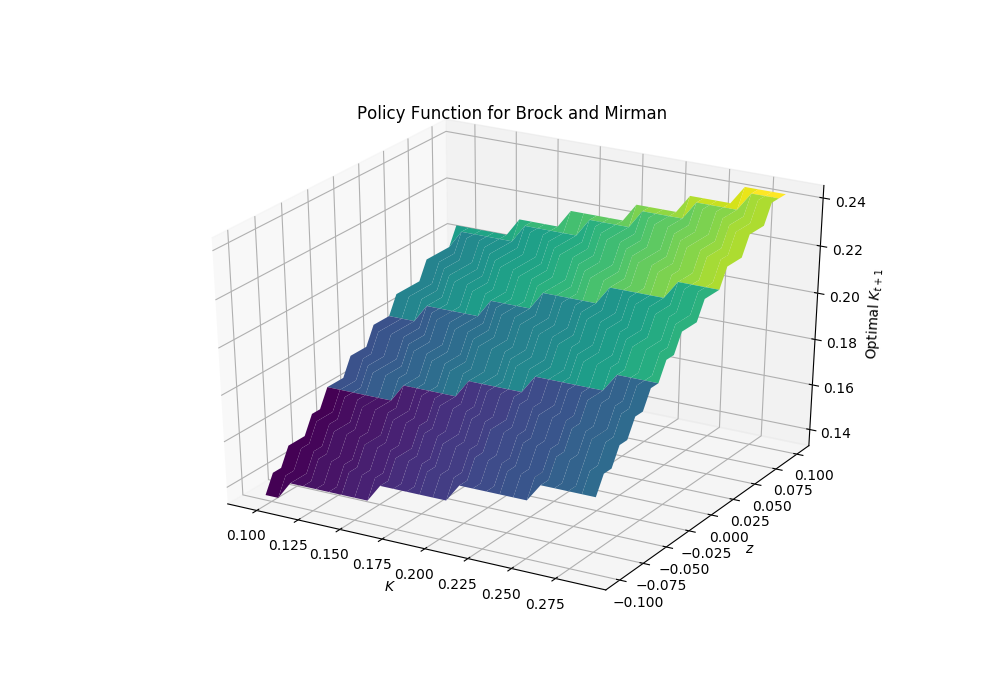
\includegraphics[width=\textwidth]{Brock_and_Merman_policy.png}
		\end{figure}
	\end{Exercise}

\section*{Linearization}\label{Linear_HW}

	\setcounter{Exercise}{0}
	% 1
	\begin{Exercise} \label{Linear_HW_BM_Coeffs}
		Using section 1.4 and the fact that $\bar{K} = A^{\frac{1}{1-\alpha}} = (\alpha\beta)^{\frac{1}{1-\alpha}}$, we have that:

		\begin{align*}
			F &= \frac{\alpha\beta\bar{K}^{\alpha-1}}{\bar{K}^\alpha-\bar{K}} = 2.708 \\
			G &= -F(\alpha+\bar{K}^{\alpha-1}) = -8.843 \\
			H &= F(\alpha\bar{K}^{\alpha-1}) = 2.763 \\
			L &= -F\bar{K} = -0.522\\
			M &= F(\bar{K}^\alpha) = 1.522 \\
			N &= \rho - 0.95
		\end{align*}

		Now we can solve for $P$ and $Q$:
		\begin{align*}
			P &= \frac{-G \pm \sqrt{G^2-4FH}}{2F} = 0.35 \\
			Q &= -\frac{LN+M}{FN+FP+G} = 0.193
		\end{align*}

		Using the following linearized policy function $K_{t+1} = H(K_t,z_t) \bar{K}+P(K_t-\bar{K})+Qz_t$, we plot the three dimensional surface plot:

		\begin{figure}[H]
			\caption{Linearized Policy Function Given Current Capital Stock and Productivity Compared with Closed Form}
			\label{fig:brock_and_mirman}
			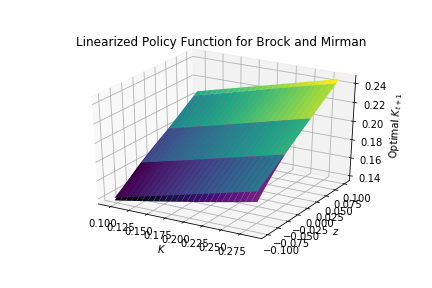
\includegraphics[width=0.8\textwidth]{Brock_and_Merman_linearized_policy.png}
		\end{figure}

		As seen, the linearized policy function intersects the real policy function (magma color scheme) at around the steady state ($K \approx 0.19, z = 0$) but deviates slightly at the non-linear parts.
	\end{Exercise}

	% 2
	\begin{Exercise} \label{Linear_HW_BM_Coeffs_Log}
		We replace all values of $K$ in the Euler Equation with $e^k$. When taking the log-linearization of the new Euler Equation we get the following matrix values:
		\begin{align*}
			F&= -0.380254 \\
			G&= 0.468559 \\
			H&= -0.117414 \\
			L&= 2.569321 \\
			M&= -2.266718 \\
			N&=0.95 \\
			P&= 0.35 \\
			Q&= 6.756849
		\end{align*}
	\end{Exercise}

	% 3
	\begin{Exercise} \label{Linear_HW_Algebra}
		Using the fact that $E\{\varepsilon_t\}=0$, we substitute equations (6), $\tilde{Z_t}=N\tilde{Z}_{t-1}$, and (7), $\tilde{X_t} = P\tilde{X}_{t-1}+Q\tilde{Z_t}$, into equation (5):
		\begin{align*}
			0 &= E_t\{F\tilde{X}_{t+1}+G\tilde{X_t}+H\tilde{X}_{t-1}+L\tilde{Z}_{t+1}+M\tilde{Z_t}\} \\
			&= FP\tilde{X_t}+FQN\tilde{Z}_{t}+GP\tilde{X}_{t-1}+GQ\tilde{Z_t}+H\tilde{X}_{t-1}+LN\tilde{Z}_{t}+M\tilde{Z_t} \\
			&= FPP\tilde{X}_{t-1}+FPQ\tilde{Z_t}+FQN\tilde{Z}_{t}+GP\tilde{X}_{t-1}+GQ\tilde{Z_t}+H\tilde{X}_{t-1}+LN\tilde{Z}_{t}+M\tilde{Z_t}\\
			&= [(FP+G)P+H]\tilde{X}_{t-1}+[(FQ+L)N+(FP+G)Q+M]\tilde{Z_t}
		\end{align*}
	\end{Exercise}

	% 4
	\begin{Exercise} \label{Linear_HW_Base_Numer_SS}
		Note that in the steady state, $\bar{z} = 0$. Therefore, there is no uncertainty and the steady states when solved numerically are (this is the same as the DSGE exercise):
		\begin{align*}
			k&=4.225, \quad \ell= 0.580, \quad r= 0.121, \quad w=1.328, \quad c=0.861, \quad T=0.043, \quad y=1.283, \quad i=0.423
		\end{align*}
	\end{Exercise}

	% 5
	\begin{Exercise} \label{Linear_HW_Base_Numer_Deriv}
			Using a first order central difference to estimate the derivatives, we have the following derivative matrix in the jupyter notebook output (refer to problem 5).
	\end{Exercise}

	% 6
	\begin{Exercise} \label{Linear_HW_Base_Coeffs}

			In order to coincide with the problem, we will use  $X_t = \{k_t,\ell_{t-1}\}$. In which case, the Uhlig's matrices are (for the log-linearized problem):
			\[
				F =
				\begin{bmatrix}
					-17.857 & 3.155\\
					0 & 0
				\end{bmatrix}
			\]

			\[
				G =
				\begin{bmatrix}
					36.196 & -3.254\\
					-22.527 & 8.638
				\end{bmatrix}
			\]

			\[
				H =
				\begin{bmatrix}
					-18.24 & 0 \\
					22.277 & 0
				\end{bmatrix}
			\]

			\[
				L =
				\begin{bmatrix}
					3.155 \\
					0
				\end{bmatrix}
			\]

			\[
				M =
				\begin{bmatrix}
					-3.254 \\
					3.004
				\end{bmatrix}
			\]

			\[
				P =
				\begin{bmatrix}
					0.915 & 0 \\
					-0.192 & 0
				\end{bmatrix}
			\]

			\[
				Q =
				\begin{bmatrix}
					0.129\\
					-0.011
				\end{bmatrix}
			\]
	\end{Exercise}

	% 7
	\begin{Exercise} \label{Linear_HW_Base_Sims}
		\begin{figure}[H]
			\caption{GDP after 10,000 Simulations}
			\label{fig:GDP_10000}
			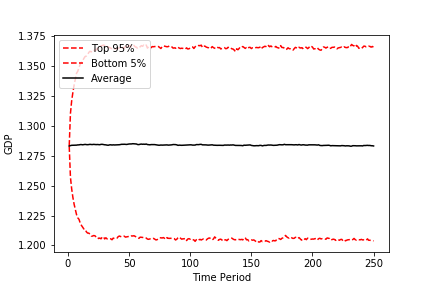
\includegraphics[width=0.7\textwidth]{GDP.png}
		\end{figure}

		\begin{figure}[H]
			\caption{Consumption after 10,000 Simulations}
			\label{fig:consumption_10000}
			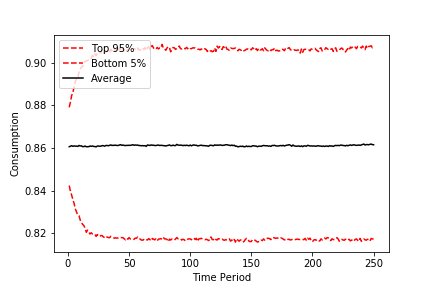
\includegraphics[width=0.7\textwidth]{consumption.png}
		\end{figure}

		\begin{figure}[H]
			\caption{Investment after 10,000 Simulations}
			\label{fig:investment_10000}
			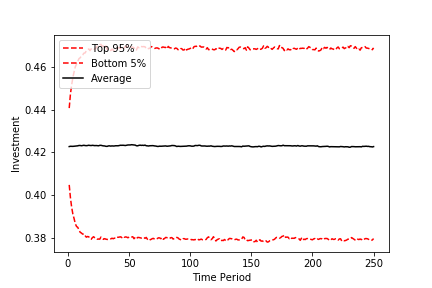
\includegraphics[width=0.7\textwidth]{investment.png}
		\end{figure}

		\begin{figure}[H]
			\caption{Labor after 10,000 Simulations}
			\label{fig:labor_10000}
			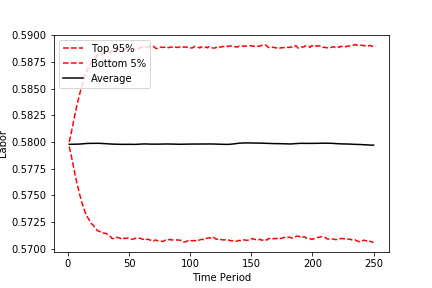
\includegraphics[width=0.7\textwidth]{labor.png}
		\end{figure}
	\end{Exercise}

	% 8
	\begin{Exercise} \label{Linear_HW_Base_Moments}
			Please refer to the juputer notebook for the result with all the moments.
	\end{Exercise}

	% 9
	\begin{Exercise} \label{Linear_HW_Base_IRFs}
		\begin{figure}[H]
			\caption{Impulse Response of GDP}
			\label{fig:GDP_impulse}
			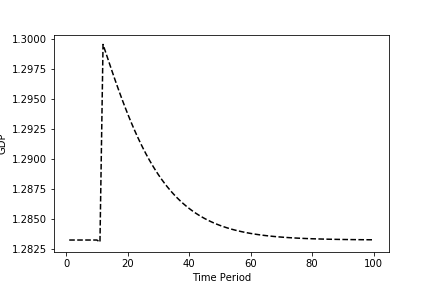
\includegraphics[width=0.7\textwidth]{GDPimpulse.png}
		\end{figure}

		\begin{figure}[H]
			\caption{Impulse Response of Consumption}
			\label{fig:consumption_impulse}
			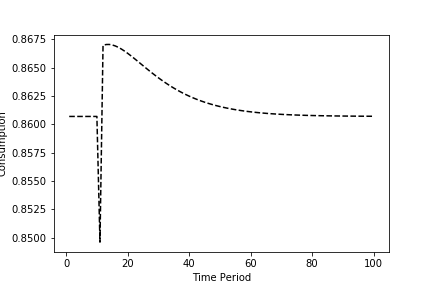
\includegraphics[width=0.7\textwidth]{Consumptionimpulse.png}
		\end{figure}

		\begin{figure}[H]
			\caption{Impulse Response of Investment}
			\label{fig:investment_impulse}
			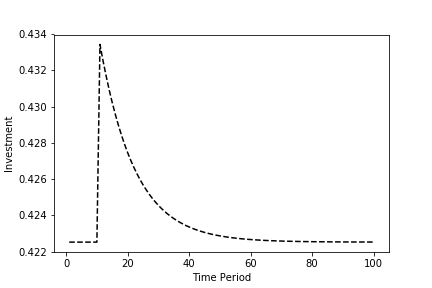
\includegraphics[width=0.7\textwidth]{Investmentimpulse.png}
		\end{figure}

		\begin{figure}[H]
			\caption{Impulse Response of Labor}
			\label{fig:labor_impulse}
			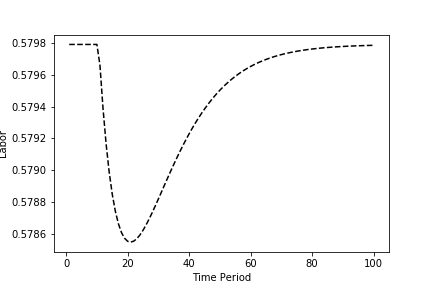
\includegraphics[width=0.7\textwidth]{Laborimpulse.png}
		\end{figure}
	\end{Exercise}

	% 10
	\begin{Exercise} \label{Linear_HW_OLG}
			\begin{figure}[H]
				\caption{Transition Path for K2}
				\label{fig:k2_tpi}
				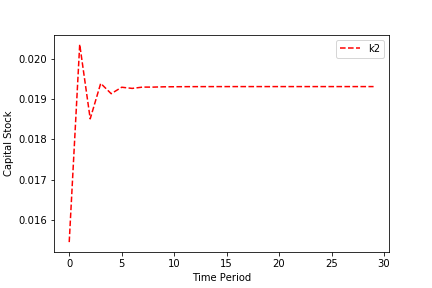
\includegraphics[width=0.7\textwidth]{k2TPI.png}
			\end{figure}

			\begin{figure}[H]
				\caption{Transition Path for K3}
				\label{fig:k3_tpi}
				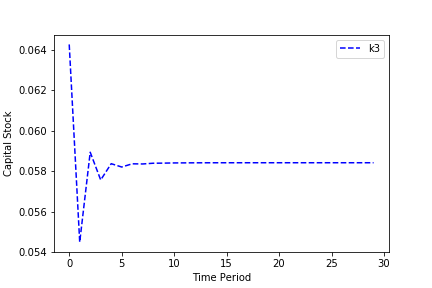
\includegraphics[width=0.7\textwidth]{k3TPI.png}
			\end{figure}

			\begin{figure}[H]
				\caption{Transition Path for K (Capital Stock)}
				\label{fig:K_tpi}
				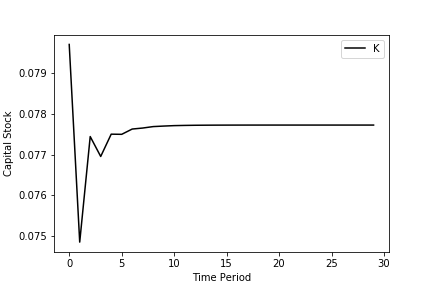
\includegraphics[width=0.7\textwidth]{KTPI.png}
			\end{figure}

			The graph for capital stock is very similar to the time path iteration result for capital, thus the linear approximation seems to be a good one. In this case, since the compute time is faster and more straight forward, it is a good tradeoff between accuracy and compute time.
	\end{Exercise}

	% 11
	\begin{Exercise} \label{Linear_HW_OLG_Stoch}
		\begin{figure}[H]
			\caption{GDP for OLG after 10,000 Simulations}
			\label{fig:GDP_OLG}
			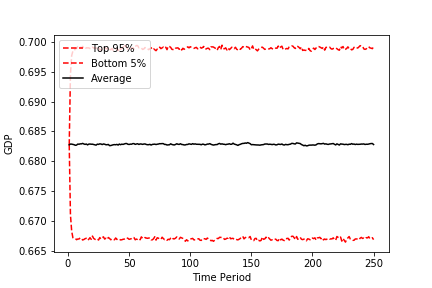
\includegraphics[width=0.7\textwidth]{GDP_OLG.png}
		\end{figure}

		\begin{figure}[H]
			\caption{Consumption for OLG after 10,000 Simulations}
			\label{fig:Consumption_OLG}
			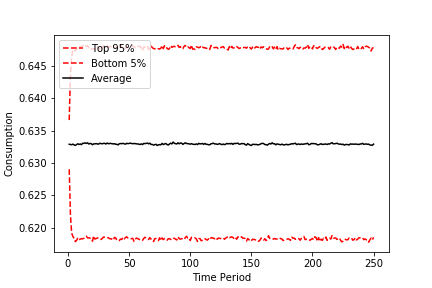
\includegraphics[width=0.7\textwidth]{Consumption_OLG.png}
		\end{figure}

		\begin{figure}[H]
			\caption{Investment for OLG after 10,000 Simulations}
			\label{fig:Investment_OLG}
			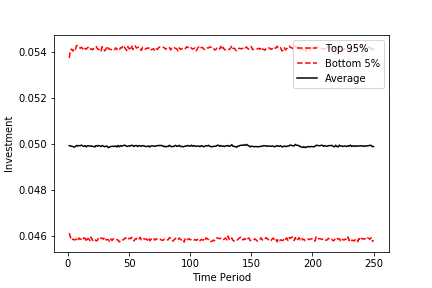
\includegraphics[width=0.7\textwidth]{Investment_OLG.png}
		\end{figure}
	\end{Exercise}

\section*{Perturbation}\label{Perturb_HW}
\setcounter{Exercise}{0}
	% 1
	\begin{Exercise} \label{Perturb_HW_Cubic}
			For the sake of clarity, we will suppress the function arguments. After deriving equation (5) again with respect to $u$ we have that:

			\begin{align*}
				x_{uuu}(u) = - \frac{F_{xxx}x_u^3 + 3(F_{xxu}x_u^2+F_{xx}x_{uu}x_u+F_{xuu}x_u+F_{xu}x_{uu})+F_{uuu}}{F_x}
			\end{align*}
	\end{Exercise}

	% 2
	\begin{Exercise} \label{Perturb_HW02_GEApprox}
		The market clearing wage rate at $k=5$ is $0.63$. The first and second order approximations are as given:

		\begin{figure}[H]
			\caption{Approximation About k=5}
			\label{fig:approx_5}
			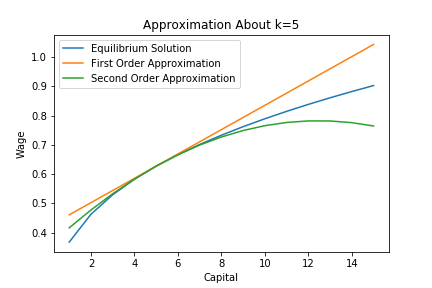
\includegraphics[width=0.8\textwidth]{approx_k_5.png}
		\end{figure}

		\begin{figure}[H]
			\caption{Approximation About k=10}
			\label{fig:approx_10}
			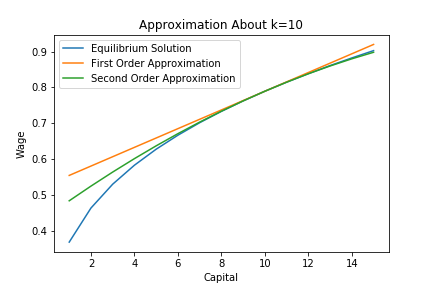
\includegraphics[width=0.8\textwidth]{approx_k_10.png}
		\end{figure}
	\end{Exercise}

	% 3
	\begin{Exercise} \label{Perturb_HW_Bivar_Grid}
		Simplifying the function and plugging in $y=G(x)$, we have the following functional form:
		\begin{equation*}
			0.95G(x)^{0.35}+1.855G(x) = x^{0.35}+0.9x
		\end{equation*}

		We have the following first, second, and third order approximations and their respective differences from the actual solution:

		\begin{figure}[H]
			\caption{Approximation About x=100}
			\label{fig:approx_F}
			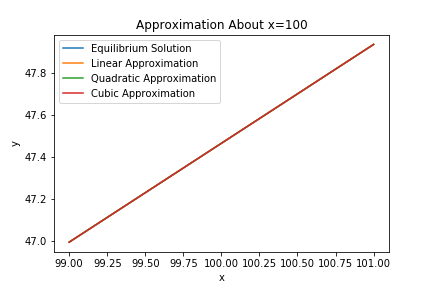
\includegraphics[width=0.8\textwidth]{approx_F.png}
		\end{figure}

		\begin{figure}[H]
			\caption{Difference from Solution}
			\label{fig:approx_diff}
			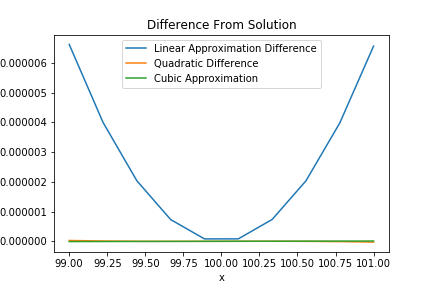
\includegraphics[width=0.8\textwidth]{approx_diff.png}
		\end{figure}
	\end{Exercise}

	% 4
	\begin{Exercise} \label{Perturb_HW_BM_NoStoch}
		From the linearization exercises, we know the analytical forms of the following derivatives (function arguments have been suppresed for clarity):
		\begin{align*}
			F_y &= F = \frac{\alpha\beta\bar{K}^{\alpha-1}}{\bar{K}^\alpha-\bar{K}} = 2.708 \\
			F_x &= G = -F(\alpha+\bar{K}^{\alpha-1}) = -8.843 \\
			F_u &= H = F(\alpha\bar{K}^{\alpha-1}) = 2.763 \\
			x_u &= P = \frac{-G \pm \sqrt{G^2-4FH}}{2F} = 0.35
		\end{align*}

		Taking the analytical derivatives, we have the following forms for the second derivatives:
		\begin{align*}
			F_{yy} &= \frac{2\alpha\beta\bar{K}^{\alpha-1}}{(\bar{K}^\alpha-\bar{K})^2} = 14.667\\
			F_{yx} &= \frac{\alpha\beta\bar{K}^\alpha(\bar{K}^{\alpha-1}(1-(\alpha+1)\bar{K}^{\alpha-1})+\alpha)}{(\bar{K}^\alpha-\bar{K})^3}=-31.431 \\
			F_{yu} &= \frac{\alpha^2\beta\bar{K}^{2(\alpha-1)}}{(\bar{K}^\alpha-\bar{K})^2} =7.483 \\
			F_{xx} &= \frac{\alpha\beta\bar{K}^\alpha(2\bar{K}^{3(\alpha-1)}+(\alpha^2+3\alpha-4)\bar{K}^{2(\alpha-1)}-2(2\alpha-1)\bar{K}^{\alpha-1}-\alpha(\alpha-1))}{(\bar{K}^\alpha-\bar{K})^3} = 105.309\\
			F_{xu} &=  -\frac{\alpha^2\beta\bar{K}^{2(\alpha-1)}(\bar{K}^{\alpha-1}+\alpha-1)}{(\bar{K}^\alpha-\bar{K})^2} = -16.953\\
			F_{uu} &= \frac{(\alpha-1)\alpha^2\beta\bar{K}^{2\alpha-3}}{\bar{K}^\alpha-\bar{K}} = -9.317
		\end{align*}

		Now we can find $x_{uu}$ using equation (12):
		\begin{align*}
			x_{uu} &=-\frac{F_{yy}x_u^4+2F_{yx}x_u^3+2F_{yu}x_u^2+F_{xx}x_u^2+2F_{xu}x_u+F_{uu}}{F_yx_u^2+F_yx_u+F_x} \\
			&= -\frac{14.667\times 0.35^4-2\times 31.431\times 0.35^3+2\times 7.483\times 0.35^2+105.309\times 0.35^2-2\times 16.953\times 0.35-9.317}{2.708\times 0.35^2+ 2.708\times 0.35-8.843} \\
			&= -1.18
		\end{align*}

		Therefore $H_X = x_u = 0.35$ and $H_{XX} = x_{uu} = -1.18$. Using the approximate policy function $K_{t+1}=\bar{K}+x_u(K_t-\bar{K})+0.5x_{uu}(K_t-\bar{K})^2$, we have:

		\begin{figure}[H]
			\caption{Brock and Mirman Second Order}
			\label{fig:BM_second}
			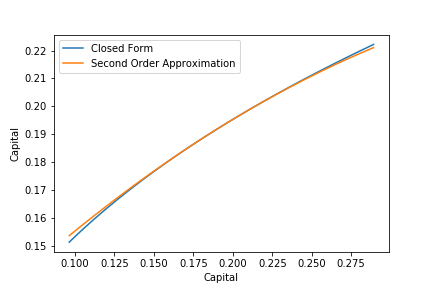
\includegraphics[width=0.8\textwidth]{BM_secondorder.png}
		\end{figure}
	\end{Exercise}

	% 5
	\begin{Exercise} \label{Perturb_HW_BM}
		Taking numerical derivatives and finding the Jacobian and Hessian of $\Gamma$, we have solve for the following values:
		\begin{align*}
			H_X &= 0.35 \\
			H_Z &= 0.1928 \\
			H_v &= 0 \\
			H_{XX}&= -1.18 \\
			H_{XZ} &= 0.35 \\
			H_{ZZ}&= 0.1827 \\
			H_{vv}&= -2.8\times10^{-17}
		\end{align*}

		We now have the second order approximation of the policy function, which we plot:
		\begin{equation*}
			K_{t+1}=\bar{K}+H_X(K_t-\bar{K})+H_Zz_t+\frac{1}{2}(H_{XX}(K_t-\bar{K})^2+H_{ZZ}z_t^2)+H_{XZ}(K_t-\bar{K})z_t+H_{vv}
		\end{equation*}

		\begin{figure}[H]
			\caption{Brock and Mirman Second Order Approximation}
			\label{fig:BM_stochastic_second}
			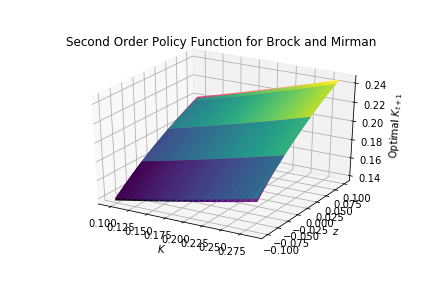
\includegraphics[width=0.8\textwidth]{Brock_and_Merman_second_order_policy.png}
		\end{figure}

		As seen compared to the actual policy function (which is underneath in purple, barely visible), it approximates the ends better than the linear approximation since the second order approximation is more appropriately curved at the ends.
	\end{Exercise}

\section*{Filtering}\label{Filter_HW}
\setcounter{Exercise}{2}

    % 3
    \begin{Exercise} \label{Filter_HW_Periodograms}
        We use U.S. quarterly and seasonally adjusted data, in billions of chained 2009 dollars, and plot the natural log of the periodogram to get the spectral density estimates from 1960 to 2017.

				\begin{figure}[H]
					\caption{Real GDP}
					\label{fig:real_GDP}
					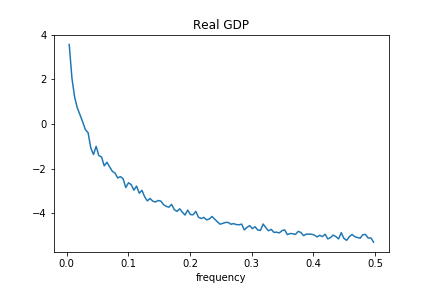
\includegraphics[width=0.8\textwidth]{Real_GDP_Periodogram.png}
				\end{figure}

				\begin{figure}[H]
					\caption{Real Personal Consumption}
					\label{fig:real_PC}
					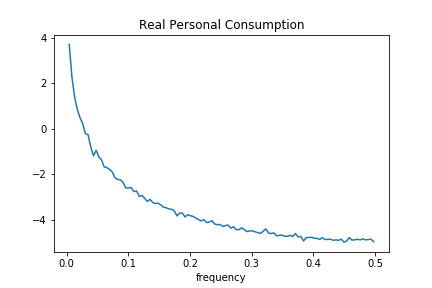
\includegraphics[width=0.8\textwidth]{Real_PC_Periodogram.png}
				\end{figure}

				\begin{figure}[H]
					\caption{Real Gross Private Domestic Investment}
					\label{fig:real_IN}
					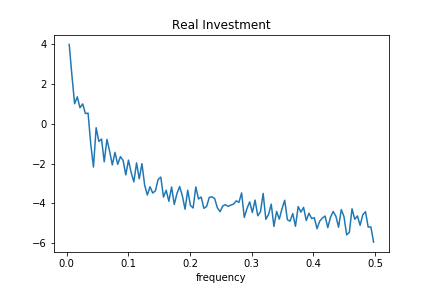
\includegraphics[width=0.8\textwidth]{Real_IN_Periodogram.png}
				\end{figure}

				\begin{figure}[H]
					\caption{Implicit GDP Deflator}
					\label{fig:GDP_deflator}
					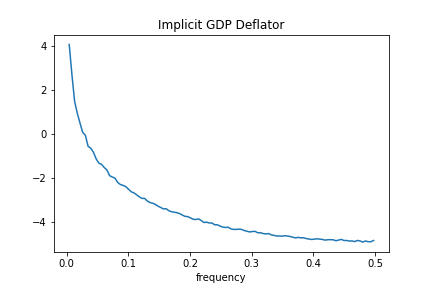
\includegraphics[width=0.8\textwidth]{Real_GDPD_Periodogram.png}
				\end{figure}
    \end{Exercise}

    % 4
    \begin{Exercise} \label{Filter_HW_Periodograms_Filtered}
        We plot the spectral estimates for first the cyclical then the trend parts of the HP-filtered time series:

				\begin{figure}[H]
					\caption{Real GDP Cyclical}
					\label{fig:real_GDPcy}
					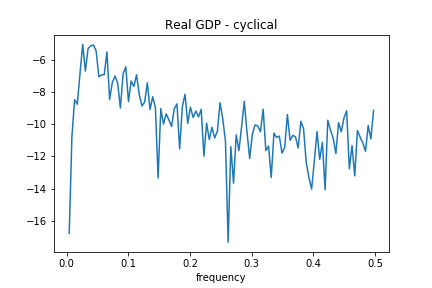
\includegraphics[width=0.8\textwidth]{Real_GDP_Cyclical.png}
				\end{figure}

				\begin{figure}[H]
					\caption{Real Personal Consumption Cyclical}
					\label{fig:real_PCcy}
					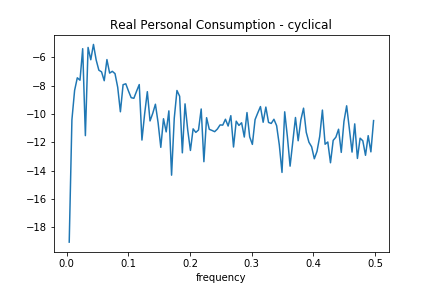
\includegraphics[width=0.8\textwidth]{Real_PC_Cyclical.png}
				\end{figure}

				\begin{figure}[H]
					\caption{Real Gross Private Domestic Investment Cyclical}
					\label{fig:real_INcy}
					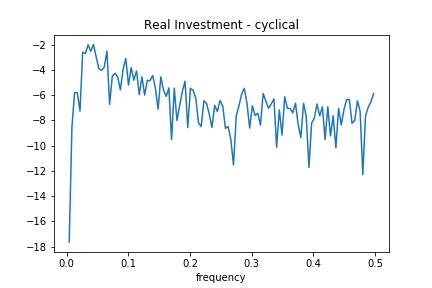
\includegraphics[width=0.8\textwidth]{Real_IN_Cyclical.png}
				\end{figure}

				\begin{figure}[H]
					\caption{Implicit GDP Deflator Cyclical}
					\label{fig:GDP_deflatorcy}
					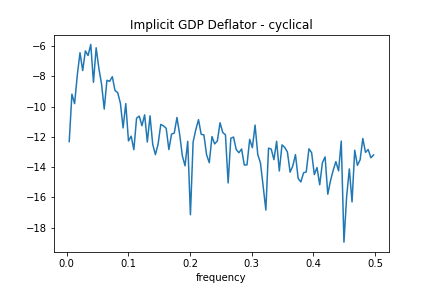
\includegraphics[width=0.8\textwidth]{Real_GDPD_Cyclical.png}
				\end{figure}

				\begin{figure}[H]
					\caption{Real GDP Trend}
					\label{fig:real_GDPtr}
					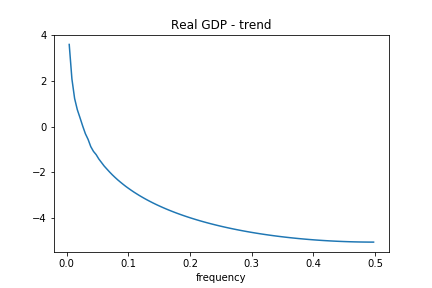
\includegraphics[width=0.8\textwidth]{Real_GDP_Trend.png}
				\end{figure}

				\begin{figure}[H]
					\caption{Real Personal Consumption Trend}
					\label{fig:real_PCtr}
					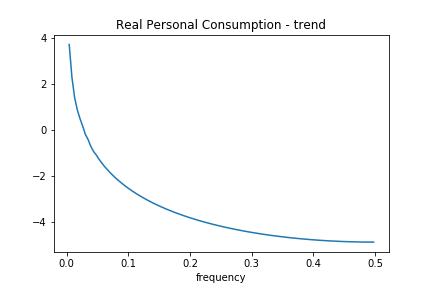
\includegraphics[width=0.8\textwidth]{Real_PC_Trend.png}
				\end{figure}

				\begin{figure}[H]
					\caption{Real Gross Private Domestic Investment Trend}
					\label{fig:real_INtr}
					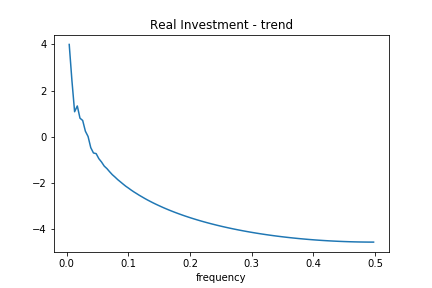
\includegraphics[width=0.8\textwidth]{Real_IN_Trend.png}
				\end{figure}

				\begin{figure}[H]
					\caption{Implicit GDP Deflator Trend}
					\label{fig:GDP_deflatortr}
					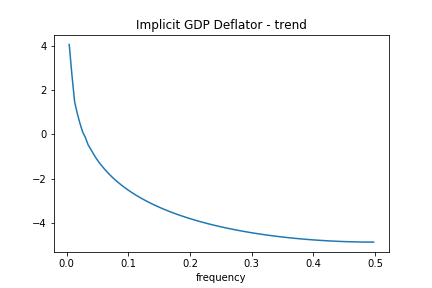
\includegraphics[width=0.8\textwidth]{Real_GDPD_Trend.png}
				\end{figure}
    \end{Exercise}

    % 5
    \begin{Exercise} \label{Filter_HW_Moments_HP}
        Please refer to the jupyter notebook for the standard deviation, autocorrelation, and correlation with GDP results for each time series and corresponding $\lambda$. Note that the standard deviation and correlation with GDP decrease as $\lambda$ increases, while autocorrelation increases as $\lambda$ increases.

				\begin{figure}[H]
					\caption{Real Investment HP-Filter $\lambda=100$}
					\label{fig:real_IN100}
					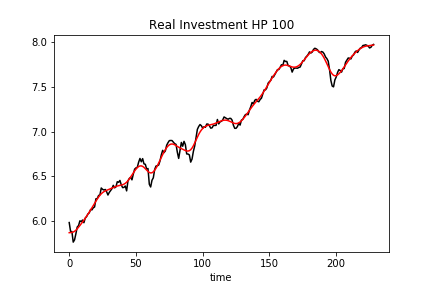
\includegraphics[width=0.8\textwidth]{Real_IN_HP100.png}
				\end{figure}

				\begin{figure}[H]
					\caption{Real Investment HP-Filter $\lambda=400$}
					\label{fig:real_IN400}
					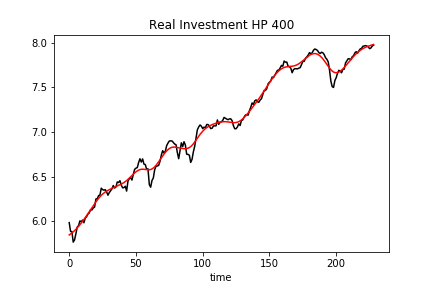
\includegraphics[width=0.8\textwidth]{Real_IN_HP400.png}
				\end{figure}

				\begin{figure}[H]
					\caption{Real Investment HP-Filter $\lambda=1600$}
					\label{fig:real_IN1600}
					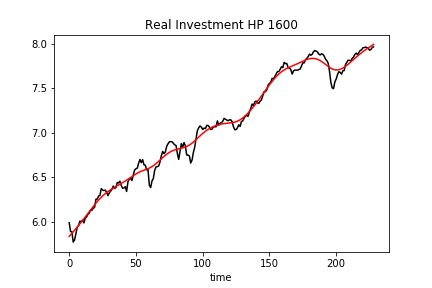
\includegraphics[width=0.8\textwidth]{Real_IN_HP1600.png}
				\end{figure}

				\begin{figure}[H]
					\caption{Real Investment HP-Filter $\lambda=6400$}
					\label{fig:real_IN6400}
					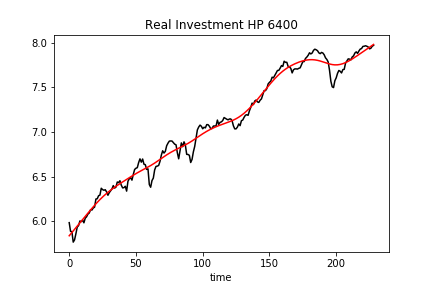
\includegraphics[width=0.8\textwidth]{Real_IN_HP6400.png}
				\end{figure}

				\begin{figure}[H]
					\caption{Real Investment HP-Filter $\lambda=25600$}
					\label{fig:real_IN25600}
					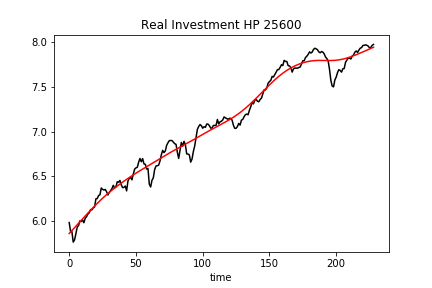
\includegraphics[width=0.8\textwidth]{Real_IN_HP25600.png}
				\end{figure}
    \end{Exercise}

    % 6
    \begin{Exercise} \label{Filter_HW_Moments}
        Replicate Table \ref{Stylized_USData_Tab} using data collected from the sites mentioned in Section \ref{Sec_FindData}.  Use quarterly data going back as far as 1947, if possible.  Do this for each of the following filters:
        \begin{itemize}
          \setlength\itemsep{0em}
          \item A linear trend filter
          \item the first difference ($y_t - y_{t-1}$) filter
          \item HP($\lambda=1600$)
          \item BP(6,32,$K=8$)
        \end{itemize}
    \end{Exercise}

\end{spacing}

\end{document}
